\documentclass{article}
\usepackage[margin=1.in]{geometry}
\usepackage[style=authoryear, 
backend=biber, 
giveninits=true,
uniquelist = false, 
uniquename=init,
isbn=false, 
maxcitenames=3,
dashed=false, 
maxbibnames=999,
doi=false,
url=false]{biblatex}
\addbibresource{biblatex-examples.bib}
\DeclareDelimFormat{nameyeardelim}{\addcomma\space}
\DeclareNameAlias{sortname}{family-given}
\renewcommand*{\labelnamepunct}{\addspace}
\DeclareFieldFormat
  [article,inbook,incollection,inproceedings,patent,thesis,unpublished]
  {title}{#1}
\DeclareFieldFormat{titlecase}{\MakeSentenceCase*{#1}}
\renewbibmacro*{in:}{%
  \ifentrytype{article}
    {\setunit{\addcomma\space}}
    {\printtext{\bibstring{in}\intitlepunct}}}
\DeclareFieldFormat{journaltitlecase}{#1}
\renewbibmacro*{journal}{%
  \ifboolexpr{
    test {\iffieldundef{Journal}}
    and
    test {\iffieldundef{journalsubtitle}}
  }
    {}
    {\printtext[journaltitle]{%
       \printfield[journaltitlecase]{journaltitle}%
       \setunit{\subtitlepunct}%
       \printfield[journaltitlecase]{journalsubtitle}}}}
\renewbibmacro*{volume+number+eid}{%
  \printfield{volume}%
  \setunit{\addcomma\space}%
  \printfield{eid}}
\DeclareFieldFormat[article,periodical]{volume}{\mkbibbold{#1}}% volume of a journal
\DeclareFieldFormat{pages}{#1}
\usepackage{amsmath,amssymb,amsfonts}
\usepackage{algorithmic}
\usepackage{graphicx}
\usepackage{textcomp}
\usepackage{xcolor}
\usepackage[font=small,labelfont=bf]{caption}
\usepackage{mathrsfs}
\usepackage{hyperref}
\usepackage{varwidth}
\DeclareMathOperator{\Loss}{\mathscr{L}}
\DeclareMathOperator{\R}{\mathbb{R}}
\DeclareMathOperator{\E}{{\text{E}}}
\DeclareMathOperator{\Var}{\text{Var}}
\DeclareMathOperator{\Cov}{\text{Cov}}
\DeclareMathOperator{\convplim}{\xrightarrow{p}}
\DeclareMathOperator{\convdlim}{\xrightarrow{d}}
\DeclareMathOperator{\plim}{\text{plim}}
\DeclareMathOperator{\GRU}{\text{GRU}}
\DeclareMathOperator{\softmax}{\text{softmax}}
\DeclareMathOperator{\attention}{\text{attention}}
\DeclareMathOperator{\mha}{\text{mha}}
% \numberwithin{equation}{section}
\usepackage{algorithm}
\usepackage{algorithmic}

\makeatletter
\@addtoreset{equation}{section}
\makeatother
\numberwithin{equation}{subsection}

\linespread{1.25}

%---MAIN---%
\begin{document}
\section{Introduction}
\subsection{GRU}

Modifying architectures to include transformers has lead to dramatic gains in many domains.
For this project, I wanted to see if I could adapt a transformer to work with a GRU.

GRU's have a simple architecture. They take in a hidden state and an input to generate 
a new state. There structure is graphically depicted in figure \ref{fig:gru-cell}.

\begin{center}
  \begin{tabular}{cc}
    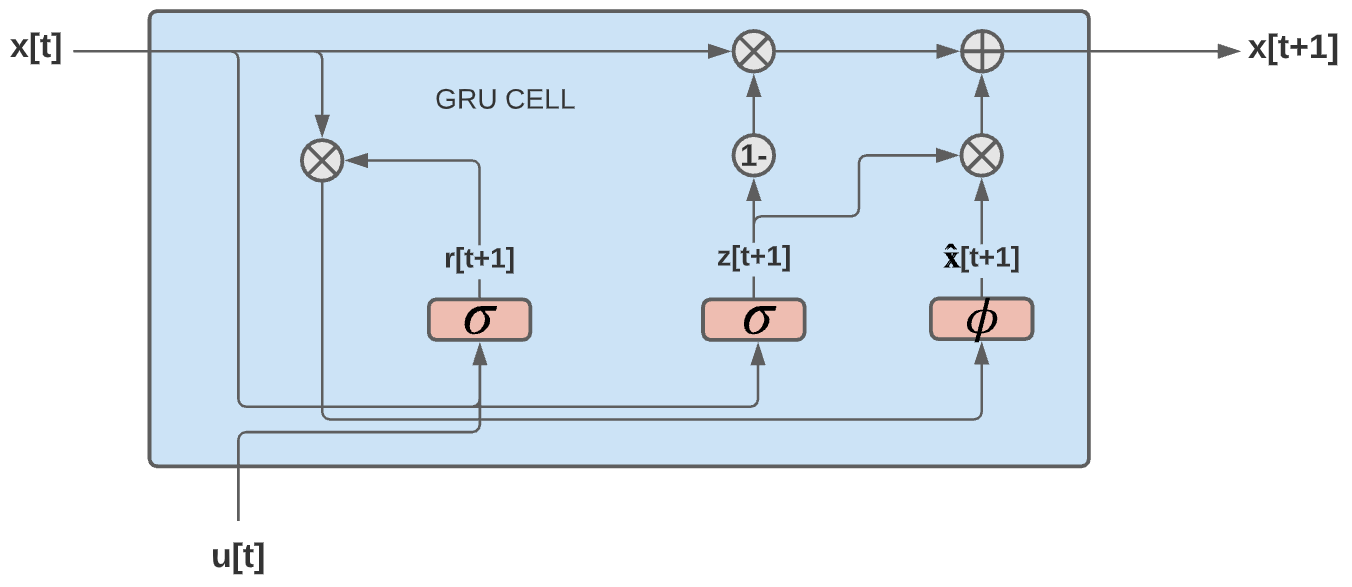
\includegraphics[width=.8\linewidth]{./figures/00-gru-cell}
  \end{tabular}
  \captionof{figure}{GRU Cell.} \label{fig:gru-cell}
\end{center}

Mathematically, a GRU Cell is described exactly as:

\begin{align}
  \begin{split}
    z[t+1] &= \sigma ( A_z x[t] + B_z u[t] + b_z) \\ 
    r[t+1] &= \sigma ( A_r x[t] + B_r u[t] + b_r) \\
    \hat x[t+1] &= \phi( A_h(r[t+1] \odot x[t]) + B_h u[t] + b_h) \\
    x[t+1] &= (1-z[t+1]) \odot x[t] + z_t \odot \hat x[t+1]
  \end{split} \label{eq:gru-cell}
\end{align}


And the elements come from the following space $x \in \R^n$, $u \in \R^m$,
$A \in \R^{n \times n}$, $B \in \R^{n \times m}$, and $b \in R^n$. Note that the vectors $b$ are optional and referred to as ``biases''.

The operations are defined as follows:

\begin{align*}
  &\sigma(x) = \cfrac{e^x}{e^x + 1} = \text{sigmoid}\\
  &\phi(x) = \cfrac{e^{2x}-1}{e^{2x} + 1} = \text{hyperbolic tangent} \\ 
  &\odot = \text{Hadamard Product (element-wise multiplication)}
\end{align*}

For simplicity, let's let $\GRU(u[t], x[t]) = x[t+1]$ represent \ref{eq:gru-cell}. We see that
while $\GRU(\cdot)$ is flexible, it has restrictive bounds on what transformations it can do to
$x[t]$ when generating $x[t+1]$. While these restrictions on $x[t+1]$ act as a regularizer, it
may prevent the GRU from tracking important features in temporal data.

\subsection{Transformers}

Transformers have produced SOTA results for sequencial data. Generaly speaking, transformers are very flexible
and while that implies they can fit many output spaces, they also require a lot of data to prevent overfitting.

Transformers work largely through a mechanism called multi-headed self-attention.

While attention is introduced in the literature in a different form, attention is
described mathematically as:

\begin{align}
  \attention(x) = \softmax \left(\frac{x M x'}{\alpha}\right)xW \label{eq:attention}
\end{align}

Where $x \in \R^{m \times n}$, $M \in \R^{n \times n}$, and $W \in \R^{n \times q}$ and $\alpha=\sqrt{q}$ which is a
that helps stabilize the gradient during backprop.  
\vspace{12pt}

Multihead attention implements multiple attention mechanisms in a system called ``attention heads''. A three headed
attention mechanism can be described as:
\begin{align}
  \begin{split}
      \mha(x)
        & =  \softmax\left( \begin{bmatrix}
            x & x & x 
          \end{bmatrix} \begin{bmatrix}
            M_1/a & 0   &  0 \\
            0   & M_2/a &  0 \\
            0   & 0   & M_3/a
          \end{bmatrix} \begin{bmatrix}
            x' & 0 & 0 \\
            0  & x'& 0 \\
            0  & 0 & x'
          \end{bmatrix}
          \right) \begin{bmatrix}
            x & 0 & 0 \\
            0 & x & 0 \\
            0 & 0 & x
          \end{bmatrix} \begin{bmatrix}
            W_1 & 0   & 0 \\
            0   & W_2 & 0 \\
            0   & 0   & W_3
          \end{bmatrix}
          U \\[5pt]
        & = \begin{bmatrix}
          \attention_1(x) & \attention_2(x) & \attention_3(x)
        \end{bmatrix}U \label{eq:mha}
  \end{split}
\end{align}
  Where $U \in \R^{n\times (3q)}$ and serves to aggregate important information found by each head.
The other matrices in  composed of unique instantiations of \ref{eq:attention}. In the generalized
case we extend the pattern seen in \ref{eq:mha} and $U \in \R^{n\times (q*h)}$.

Though transformers are flexible, they have no state variables. This means that transformers cannot
account for dynamic behavior that cannot be described by the window of input data. To overcome this,
a mechanism called time2vec was developed which, in theory, can find a multi-dimension time-embedding
to help account for time-trends in time-series data. This learned embedding has had varying degrees
of success.

\subsection{Feature RNN}

To assist a model with learning temporal features, our proposed network is the feature recurrent neural
network (FRNN). An outline of the architecture is shown in figure \ref{fig:FRNN}.

\begin{center}
  \begin{tabular}{cc}
    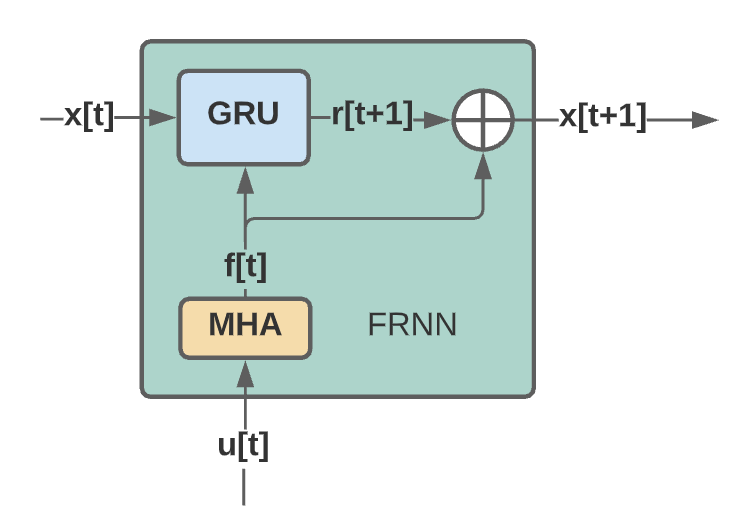
\includegraphics[width=.8\linewidth]{./figures/01-FRNN}
  \end{tabular}
  \captionof{figure}{GRU Cell.} \label{fig:FRNN}
\end{center}
The FRNN builds off its predecessors so it can be understood in $3$ steps:
\begin{enumerate}
  \item FRNN accepts a new input from which it extracts relevant time-varying features.
  \begin{align}
    \mha(u[t]) = f[t]
  \end{align}
  \item FRNN combines these new features with the hidden instate to produce a new state variable
  \begin{align}
    \GRU(x[t], u[t]) = r[t+1]
  \end{align}
  \item Attention mechanisms are data hungry, so to help gradient flow the the multi-headed attention
        unit, the hidden state is added added and normalized (not depicted) by the current extracted
        features.
        \begin{align}
          \begin{split}
            z[t]   &= f[t] + r[t+1] \\
            x[t+1] &= \frac{z_t}{\| z_t \|}
          \end{split}
        \end{align}
\end{enumerate}

\section{Results}

Training the model follows the pseudo-code outlined in \ref{alg:train}. When I initially constructed
the trianing loop, I tought that the training process would be fairly quick because I excluded the
start warmup from the gradient, however each epoch was estimated to take over 3 weeks to train with
$5,236$ batches of training data. Needless to say, this was prohibitively slow.

The next step would be to take a random sample of batches and enable multiple batches to be trained
at a time. This is a non-trivial task because the warm-up data needs to be accessible for each batch.
Perhaps this will become a summer project.

\begin{algorithm}
\caption{Training Loop} \label{alg:train}
\begin{algorithmic}
\FOR{Epoch in 1:Epochs}
  \FOR{i in 1:length(training)}
    \STATE x $\leftarrow$ Model.init\_state
    \\ 
    \COMMENT{warmup state}
    \FOR{j in 1:i}
      \STATE y, x $\leftarrow$ Model.predict(data(j), x)
    \ENDFOR
    \STATE Model.fit(data(i), x)
  \ENDFOR
\ENDFOR
\end{algorithmic}
\end{algorithm}







\ \\\ \\\  \\\  \\\  \\\  \\\  

% \textcite{sigfridsson,worman,geer,maron}

% \parencite[e.g.,][]{nussbaum,companion}

% \printbibliography

\end{document}
